\documentclass[conference,letterpaper]{IEEEtran}
\usepackage[T1]{fontenc}
\usepackage[utf8]{inputenc}
\usepackage{amsmath,amssymb}
\usepackage{graphicx}
\usepackage{cite}
\usepackage{url}
\usepackage{xurl}
\usepackage{array}
\usepackage{tikz}
\usetikzlibrary{arrows.meta,positioning,calc}
\renewcommand{\arraystretch}{1.12}
\newcommand{\code}[1]{\texttt{\footnotesize #1}}

\begin{document}

\title{UMBRA: Browser-Based Private Proximity Testing with Multiparty Homomorphic Encryption and Garbled Circuits}

\author{%
\IEEEauthorblockN{Fernanda Santill\'an Dant\'es}
\IEEEauthorblockA{\textit{School of Engineering and Sciences}\\
\textit{Tecnol\'ogico de Monterrey}\\
Monterrey, Mexico}
\and
\IEEEauthorblockN{Carlos Eduardo Arias Capetillo}
\IEEEauthorblockA{\textit{School of Engineering and Sciences}\\
\textit{Tecnol\'ogico de Monterrey}\\
Monterrey, Mexico}
\and
\IEEEauthorblockN{Alberto L\'opez Barrag\'an}
\IEEEauthorblockA{\textit{School of Engineering and Sciences}\\
\textit{Tecnol\'ogico de Monterrey}\\
Monterrey, Mexico}
\and
\IEEEauthorblockN{Juan David Guarnizo Hernandez}
\IEEEauthorblockA{\textit{School of Engineering and Sciences}\\
\textit{Tecnol\'ogico de Monterrey}\\
Monterrey, Mexico}}

\maketitle

\begin{abstract}
Location-based services are widely used in communication and e-services, and they require users to provide their location to obtain an efficient or improved outcome. However, these data can be abused, leaked or misused, as the 2024 Gravy Analytics case showed. In this work, we introduce UMBRA, a privacy-preserving web application that allows a verifier to conclude whether a location provided by a prover lies within a range of a point of interest, while the location itself is never disclosed. Both parties encrypt their locations in their browsers under a shared key that neither can decrypt alone; an untrusted server uses multiparty homomorphic encryption to compute on the encrypted data, and a garbled circuit reveals to the verifier only whether the location is inside, on the boundary of, or outside the range. We demonstrate UMBRA with a simulated police request about whether a citizen was near a crime scene. In our experiments, all 10,011 evaluations returned the correct class; the cryptography takes under a second, while a complete evaluation takes about seven seconds in the browser, mostly waiting for messages. Thus, the answer to our research question is affirmative: useful information can be derived from data that is never seen.
\end{abstract}

\begin{IEEEkeywords}
secure multiparty computation, homomorphic encryption, garbled circuits, oblivious transfer, location privacy, WebAssembly
\end{IEEEkeywords}

\section{Introduction}
Location-based services have expanded greatly within the last ten years, and the usefulness of working with accurate locations is a feature that neither the user nor the provider can ignore. However, location is one of the most private kinds of data a person creates, yet proximity questions are often answered by sharing a whole location history with anyone asking. Secure computation~\cite{yao86} provides a solution that involves less disclosure: two entities compute a predefined function of their private data and receive only the result. Homomorphic encryption~\cite{bgv}, which allows computing on encrypted data, is one such technique.

\textbf{\textit{Problem.}} Location-based services make it necessary for the user to provide accurate geographic information to intermediaries that may misuse it or be breached. In December 2024, the U.S. Federal Trade Commission brought a case against the data company Gravy Analytics on account of selling non-anonymized precise location data obtained without verifiable consent~\cite{ftc}. After a month, there was a security breach in the company's system~\cite{tc}. The conflict also exists in law enforcement: verifying whether a person was near a crime scene usually requires disclosing that person's exact location. The problem we address is providing this answer without anyone, the server included, learning the location.

\textbf{\textit{Context.}} The UMBRA scenario models a police investigation as to whether a person was close to a crime scene. Here, the Police (the verifier) have a reference point $P$ (the crime scene) and a public radius $R$, while the User (the prover) has a private location $U$. Both parties use a WebAssembly client running in their browser, implemented with the help of the Lattigo open-source library~\cite{lattigo}, and an untrusted Go server orchestrates the protocol and performs computation on encrypted data. To sum up, our solution consists of four stages. First, both the Police and the User encrypt their locations in their browsers independently using a key that is split between the two parties in such a way that neither can decrypt the message independently. Second, the server performs computation on the encrypted data without ever accessing any coordinates. Third, the resulting encrypted value is transformed, without decryption, into two seemingly random values, one for the Police and one for the User. Finally, the garbled circuit takes both values and returns to the Police whether the User's location falls inside, outside, or at the edge of the radius.

\textbf{\textit{Related work.}} Private proximity testing has been studied for more than fifteen years. Zhong et al.~\cite{zhong07} proposed three protocols that let a user learn whether a friend is nearby without revealing their locations; Narayanan et al.~\cite{narayanan11} reduced proximity testing to private equality tests over grid cells, strengthened by location tags; \v{S}ed\v{e}nka and Gasti~\cite{sedenka14} computed distances on the surface of the Earth rather than on a plane; and InnerCircle~\cite{hallgren15} is a decentralized, parallelizable protocol based on partially homomorphic encryption and secure against semi-honest adversaries. During the COVID-19 pandemic, proximity-tracing systems such as DP-3T~\cite{dp3t} estimated exposure from Bluetooth contacts between phones rather than from locations. These designs are two-party protocols between the users or rely on dedicated mobile apps. In contrast, UMBRA lets an untrusted web server compute on encrypted locations with multiparty homomorphic encryption, runs both clients unchanged in a browser, and reveals to the verifier only the class of each query.

\textbf{\textit{Justification.}} Possible answers to the problem raised by the scenario are inside, boundary and outside. In one of the initial prototypes, the margin $\Delta$ of Section~\ref{sec:function} was decrypted, allowing the exact distance and the User's position to be found after two queries (Section~\ref{sec:e10}). Revealing only the answer provides strictly less information than the distance itself and allows us to analyze its cost in a browser deployment.

\textbf{\textit{Objective.}} Replace the plaintext decryption of $\Delta$ with a garbled circuit that reveals only the classification, and evaluate the result: correctness against a plaintext reference, the limits of the encoding, the cost per participant, and what the remaining leakage is.

\textbf{\textit{Hypothesis.}} For inputs inside the supported range and parties that follow the protocol, the encrypted workflow returns the same class as a plaintext computation, and the Police obtain no more than that class from one evaluation.

The research question addressed in this work is:
\begin{quote}
\textit{Can we develop a system that enables a service provider or stakeholder to obtain business-logic outcomes from user data that stays encrypted throughout the computation?}
\end{quote}

The rest of the paper is organized as follows: Section~\ref{sec:background} reviews the cryptographic background, Section~\ref{sec:arch} describes the system, Section~\ref{sec:impl} the implementation, Section~\ref{sec:eval} the experiments, Section~\ref{sec:security} the security discussion, and Section~\ref{sec:concl} concludes.

\section{Background}\label{sec:background}
This section reviews the building blocks of UMBRA. The BGV homomorphic encryption scheme (Section~\ref{sec:bgv}) and its multiparty version (Section~\ref{sec:mpbgv}) let the server compute on encrypted locations without any party holding the full secret key. Encryption-to-shares (Section~\ref{sec:e2s}) turns the encrypted result into two random-looking shares, and a garbled circuit (Section~\ref{sec:gc}) with oblivious transfer (Section~\ref{sec:ot}) combines the shares and outputs only the class.

\subsection{BGV Homomorphic Encryption Scheme}\label{sec:bgv}
BGV~\cite{bgv} is a leveled homomorphic encryption scheme using the ring learning-with-errors problem. Specifically, we have $R_Q = (\mathbb{Z}/Q\mathbb{Z})[X]/(X^N+1)$, where $Q$ is the ciphertext modulus and $N$ is a power of two. This is the set of polynomials with coefficients in $\mathbb{Z}/Q\mathbb{Z}$ and degree less than $N$. Further, let $t$ be the plaintext modulus. The secret key is a polynomial $s \in R$ whose coefficients are small. The ciphertext is a pair $(c_0, c_1) \in R_Q^2$ satisfying
\begin{equation}
c_0 + c_1 s \equiv m + t e \pmod{Q},
\end{equation}
where $m \in R_t$ is the message and $e$ is the noise polynomial. Decryption evaluates the left-hand side, takes the centered representative modulo $Q$ and reduces it modulo $t$. The result $m$ is correct if $-Q/2 < m_i + t e_i < Q/2$ for every coefficient $i$.

The noise grows linearly with ciphertext addition. For multiplication, the noise terms are multiplied in the resulting ciphertext, which has three components. The relinearization key (RLK), an encryption of $s^2$ under an auxiliary modulus $P$, is needed to reduce the ciphertext back to two components. Each multiplication uses part of the noise budget $\log_2(Q/2) - \log_2\|m+te\|_\infty$, which is why $Q$ is chosen taking into account the multiplicative depth of the function. If $t \equiv 1 \pmod{2N}$, then $R_t$ can be divided into $N$ slots that are added and multiplied separately. The security of the scheme depends on the value of $N$ in relation to $\log_2 QP$.

\subsection{Multiparty BGV}\label{sec:mpbgv}
In the construction of Mouchet et al.~\cite{mouchet}, party $i$ holds a share $s_i$, and the secret key of the group is defined as $s = \sum_i s_i$. The collective public key (CPK) is generated in such a way that all parties use the same public random polynomial $a$ from a common reference string. Each party discloses $p_i = -a s_i + e_i$, while the key is $(\sum_i p_i, a)$. Anybody having the public key can encrypt and compute on the encrypted information. Decryption requires contributions from all parties involved, so no party can decrypt alone.

\subsection{Encryption-to-Shares}\label{sec:e2s}
Encryption-to-shares (E2S)~\cite{mouchet} replaces decryption when the plaintext needs to be kept confidential. Given a ciphertext $(c_0, c_1)$, party $i$ chooses a uniformly random mask $M_i \in R_t$ and publishes
\begin{equation}
h_i = c_1 s_i + e'_i - M_i,
\end{equation}
where $M_i$ is encoded in $R_Q$ and $e'_i$ is a fresh flooding noise that is meant to be much larger than the encryption noise to hide the noise in the ciphertext (in our parameters it is not; Section~\ref{sec:flood}). Anybody can add the public shares to $c_0$ and decrypt $m - \sum_i M_i$, which has a uniform distribution. One of the parties adds its own mask again. With two parties, the Police keep $s_P = M_P$ and the User obtains $s_U = m - M_P$, so that for the margin $\Delta$ of Section~\ref{sec:function}
\begin{equation}
s_P + s_U \equiv \Delta \pmod{t},
\end{equation}
and each share alone is uniform.

\subsection{Yao Garbled Circuits}\label{sec:gc}
A garbled circuit~\cite{yao86,bhr12} lets an evaluator compute a Boolean circuit on inputs that it cannot read. The garbler associates with each wire two random 128-bit labels representing each possible value of the wire. The evaluator owns precisely one label per wire but does not know which bit value it stands for. In the free-XOR optimization~\cite{freexor}, the difference between the two labels of each wire equals the same secret offset value, so the label of an XOR output is the XOR of the input labels and needs no ciphertext; NOT operations are free too. The garbler sends four ciphertexts for each AND gate, each one corresponding to the output label encrypted under one possible combination of the input labels, using SHA-256 as the key derivation function. The point-and-permute method~\cite{bmr90} uses one pointer bit in every label so that the evaluator knows which row to decrypt.

The circuit used here takes the two 17-bit shares, adds them modulo $t$ with a ripple-carry adder and outputs two bits: whether the centered result is negative and whether it is zero.

\subsection{Oblivious Transfer}\label{sec:ot}
The evaluator needs the labels of its input bits, but the garbler must not learn the bits, and the evaluator must not get both labels of a wire. This is a 1-out-of-2 oblivious transfer (OT): the sender has $(m_0, m_1)$, the receiver has a bit $b$ and learns only $m_b$. We follow the protocol of Chou and Orlandi~\cite{chouorlandi} over the edwards25519 group with base point $B$: the sender sends $A = aB$; for every bit, the receiver sends $R = xB + bA$; the sender encrypts $m_0$ with a key derived from $aR$ and $m_1$ with a key derived from $a(R - A)$; the receiver can only compute the key derived from $xA$. There are three messages in total, called \code{otA}, \code{otR} and \code{otE} in the prototype, and each session moves the 17 labels of the Police share.

\section{Architecture and System Model}\label{sec:arch}
\subsection{Actors and Trust Boundaries}
In one assignment there are three actors (Fig.~\ref{fig:arch}). The client of the Police holds $P = (P_x, P_y)$ and part of the secret key. The client of the User holds $U = (U_x, U_y)$ and the other part of the secret key. The server does not hold any part of the secret key; it combines public shares, evaluates the function on encrypted data and relays the circuit messages. The secret keys, coordinates and additive shares never leave the browser in which they were created. All parties are assumed semi-honest: they follow the protocol but inspect what they receive, and the server, which also enforces the quota, does not collude with either party.

\begin{figure}[t]
\centering
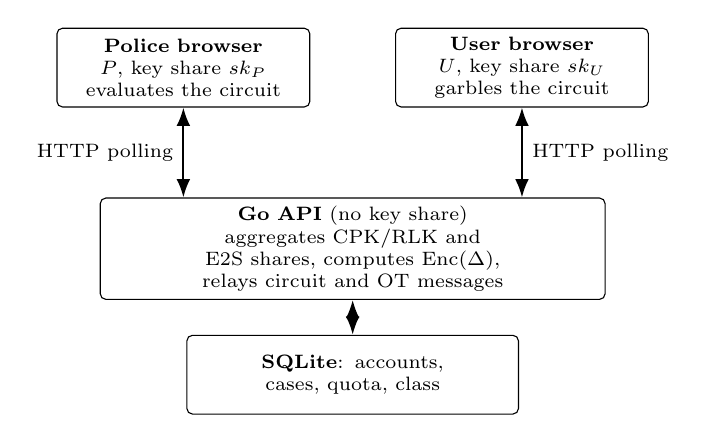
\begin{tikzpicture}[font=\scriptsize,
  box/.style={draw, rounded corners=2pt, align=center, minimum height=10mm, inner sep=3pt},
  arr/.style={Latex-Latex, thick}]
\node[box, text width=30mm] (police) at (-2.15,0) {\textbf{Police browser}\\$P$, key share $sk_P$\\evaluates the circuit};
\node[box, text width=30mm] (user) at (2.15,0) {\textbf{User browser}\\$U$, key share $sk_U$\\garbles the circuit};
\node[box, text width=62mm] (api) at (0,-2.3) {\textbf{Go API} (no key share)\\aggregates CPK/RLK and E2S shares, computes $\mathrm{Enc}(\Delta)$,\\relays circuit and OT messages};
\node[box, text width=40mm] (db) at (0,-3.9) {\textbf{SQLite}: accounts, cases, quota, class};
\draw[arr] (police.south) -- node[left]{HTTP polling} (police.south |- api.north);
\draw[arr] (user.south) -- node[right]{HTTP polling} (user.south |- api.north);
\draw[arr] (api) -- (db);
\end{tikzpicture}
\caption{Actors and communication in one assignment. Each browser box is a trust boundary: plaintext coordinates, secret-key shares and additive shares of $\Delta$ never leave it; only public shares, ciphertexts and garbled material travel over HTTP.}
\label{fig:arch}
\end{figure}

\subsection{Computed Function}\label{sec:function}
Using the public radius $R$, the server evaluates under the collective key
\begin{equation}\label{eq:delta}
\Delta = (P_x - U_x)^2 + (P_y - U_y)^2 - R^2,
\end{equation}
which requires multiplicative depth one. In this paper, $\Delta$ is the name for this margin; the global offset of the free-XOR approach, also called ``delta'' in the garbling literature, is here called the free-XOR offset.

\subsection{Steps of the Protocol}
(1)~Both clients compute key shares and participate in the CPK and two rounds of RLK generation. (2)~Both clients encrypt their two coordinates under the CPK, one ciphertext per coordinate, using only slot~0. (3)~The server computes $\mathrm{Enc}(\Delta)$ according to~\eqref{eq:delta}. (4)~Both clients execute the E2S protocol with discrete Gaussian flooding noise of standard deviation $2^{30}$ and obtain shares satisfying~(3). (5)~The User garbles a circuit that computes the sum of the two 17-bit shares modulo $t$ and returns the result as two bits, $[\Delta < 0,\ \Delta = 0]$; the Police get their input labels via oblivious transfer and evaluate the circuit to determine the class of the point: inside, boundary or outside.

\section{Implementation Details}\label{sec:impl}
\subsection{Server}
The server is a natively built Go application that uses an SQLite database; unlike the clients, it is not executed in the browser. The server authenticates the clients with tab-specific bearer tokens and stores the accounts, cases, assignments, the evaluation quota and the resulting class. It exposes the endpoints through which the setup shares, ciphertexts, E2S shares and the five circuit messages (garbled tables, garbler labels, \code{otA}, \code{otR}, \code{otE}) pass. The endpoints of the earlier version that returned a decryption of $\Delta$ have been removed.

\subsection{WebAssembly Client}
The client is the same Go code compiled with \code{GOOS=js GOARCH=wasm}. JavaScript loads the module and calls it through a single JSON entry point. A one-second timer polls the server and advances the protocol, with a guard against overlapping rounds. We chose WebAssembly so that the same cryptographic code runs unchanged in any modern browser without installing anything, and no person's location or key share leaves their own device; the cost is about 4.1 times the native time (Section~\ref{sec:e9}).

\subsection{Client State Recovery}
The state of each client (the key share, the E2S mask and the garbling secrets) is serialized in the browser's IndexedDB, keyed by session and role, before the corresponding public message is sent. Therefore, when the client reloads, it continues the current session without generating a new key share. If the state is lost, either client may start a new session and clear all the public information for this pair.

\section{Experimental Evaluation}\label{sec:eval}
\subsection{Setup and Method}
Measurements were made on one machine: HUAWEI MCLG-XX, 13th Gen Intel Core i9-13900H (14 cores, 20 threads), 15.7~GiB RAM, Microsoft Windows 11 Home Single Language (10.0.26300), go1.26.0, on 2026-11-17. Experiments are run with a native Go harness that calls the application's own packages; the HTTP server, SQLite and the browser are excluded unless explicitly mentioned. Each experiment produces one CSV row per run, and medians are reported with the interquartile range (IQR). Three warm-up runs are discarded. Time is read from the Windows performance counter because Go's monotonic clock on Windows returned 0 for sub-millisecond phases. Memory is reported as peak working set, the Windows counterpart of resident set size. The prototype uses Lattigo v6.2.0~\cite{lattigo}.

\textbf{\textit{Input domain.}} Coordinates and radius are integers in $[0, 100]$, a normalized grid, so that $\Delta \in [-10{,}000,\ 20{,}000]$. A real deployment would project GPS coordinates onto a local metric grid and choose the plaintext modulus $t$ for the required range (Section~\ref{sec:e5}).

\textbf{\textit{Measurement conditions.}} The laptop was connected to its original charger, with the Windows power mode set to Best performance, in controlled conditions with no other load. Windows Defender real-time protection was active. Random inputs and the common reference string are seeded; Lattigo's key and encryption randomness cannot be seeded. Parameter sets were timed with 30 runs each. All experiments were run once, in order; the files of an earlier run on 2026-11-12 are also kept (Appendix~\ref{app:repro}).

\subsection{Correctness (E1)}
The class returned by the protocol was compared with the plaintext class for 10,011 cases (the 11 named cases of Table~\ref{tab:e1} and 10,000 random inputs in $[0, 100]$): there were no discrepancies and no failures. The classes found were 4,760 inside, 9 boundary and 5,242 outside. The same test was executed end to end in the browser with four cases, all with $P = (10, 20)$ and $R = 5$, in headless Chrome 157.0.8103.79: all four yielded the expected result page (inside, boundary, outside, and the quota error on a fourth attempt for the same pair within one hour; Appendix~\ref{app:evidence}).

\begin{table}[t]
\caption{Correctness Cases with Named Examples (E1). $\Delta<0$ Is Inside, $\Delta=0$ Boundary and $\Delta>0$ Outside; Expected Is the Plaintext Class and Observed the Class Returned by the Encrypted Protocol.}
\label{tab:e1}
\centering
\scriptsize
\setlength{\tabcolsep}{2.4pt}
\begin{tabular}{lcccrll}
\hline
Case & $P$ & $U$ & $R$ & $\Delta$ & Expected & Observed \\
\hline
inside & (10,20) & (11,22) & 5 & $-20$ & inside & inside \\
boundary & (10,20) & (13,24) & 5 & $0$ & boundary & boundary \\
outside & (10,20) & (14,24) & 5 & $7$ & outside & outside \\
delta\_min & (0,0) & (0,0) & 100 & $-10000$ & inside & inside \\
delta\_max & (100,100) & (0,0) & 0 & $20000$ & outside & outside \\
identical\_r0 & (5,5) & (5,5) & 0 & $0$ & boundary & boundary \\
identical\_r1 & (50,50) & (50,50) & 1 & $-1$ & inside & inside \\
corners\_r100 & (0,0) & (100,100) & 100 & $10000$ & outside & outside \\
corners\_anti\_r0 & (0,100) & (100,0) & 0 & $20000$ & outside & outside \\
adjacent\_r1 & (0,0) & (0,1) & 1 & $0$ & boundary & boundary \\
adjacent\_r0 & (0,0) & (0,1) & 0 & $1$ & outside & outside \\
\hline
\end{tabular}
\end{table}

\subsection{Sign-Wrap Limit (E2)}\label{sec:e2}
Bypassing the validation performed by the client, we tested every true $\Delta$ from $-70{,}000$ to $70{,}000$ in coarse steps and all integers close to $\pm 32{,}768$ (239 tests, none crashed). The class is correct for $\Delta$ from $-32{,}768$ to $32{,}768$; the first wrong classes appear at $-32{,}769$ and $32{,}769$. This is caused by the centered representation of numbers modulo $t = 65{,}537$: a value beyond half the modulus wraps to the other sign. For values above $\pm 65{,}537$ the value wraps a full turn, and the class is correct again only by coincidence.

\subsection{Noise and Phase Times (E3)}\label{sec:e3}
During 1,011 runs (1,000 random inputs plus the 11 cases of Table~\ref{tab:e1}) with new keys every 50 runs, there were no wrong classes and no failures. For a fresh ciphertext, $|m+te|$ is about $2^{23.5}$; after the multiplication it becomes $2^{54.4}$ (maximum $2^{54.7}$), whereas the modulus has 328 bits. The noise budget left after E2S is 272.6 bits (minimum 272.3). The modulus chain is therefore much larger than a depth-one computation needs, which motivates the sweep in Section~\ref{sec:e4}. Table~\ref{tab:e3} gives the time of each phase: the lattice operations dominate, while the garbled circuit (5,322 bytes) takes only microseconds because it has few AND gates; within the circuit phase, the 17 oblivious transfers dominate.

\begin{table}[t]
\caption{Native Time per Phase in ms with the Deployed Parameters (E3; Work of Both Parties Summed Where Applicable)}
\label{tab:e3}
\centering
\scriptsize
\setlength{\tabcolsep}{3pt}
\begin{tabular}{lrrrr}
\hline
Phase & Median & IQR & Min & Max \\
\hline
Collective keygen (CPK+RLK) & 78.3 & [73.9, 83.5] & 61.5 & 101 \\
Encrypt (4 ciphertexts) & 35.2 & [33.2, 39.0] & 28.8 & 75.2 \\
Server evaluation of $\Delta$ & 61.8 & [57.9, 66.9] & 50.1 & 128 \\
Encryption-to-shares & 7.95 & [7.45, 8.99] & 6.21 & 19.6 \\
Garble & 0.0657 & [0.0597, 0.0713] & 0.0470 & 0.307 \\
Oblivious transfer (17) & 2.23 & [2.06, 2.45] & 1.55 & 9.39 \\
Circuit evaluation & 0.0122 & [0.0114, 0.0134] & 0.00860 & 0.0656 \\
\hline
\end{tabular}
\end{table}

\subsection{Parameter Sweep (E4)}\label{sec:e4}
We tested 48 parameter sets: $\log N$ from 12 to 15, six modulus chains from 109 to 438 bits, and two secret-key distributions (Lattigo's default uniform ternary distribution and ternary with a fixed Hamming weight of 192). Each set ran in a separate process with 30 timing runs, executed serially, and 1,011 correctness runs, executed on 8 parallel workers. Across the 48 sets, 47 returned the correct class in every run, one did not, and all could be instantiated.

\textbf{\textit{Security check.}} We checked $\log QP$ against the maximum modulus that the Homomorphic Encryption Standard~\cite{hestd} lists for classical 128-bit security with a uniform ternary secret (109, 218, 438 and 881 bits for $N = 2^{12}$ to $2^{15}$). The deployed set ($\log N = 14$, $\log Q = 328$, $\log P = 110$) lies exactly on this bound. The check is a lookup in a 2018 table, not a current estimation, and it does not cover the multiparty case or sparse secrets; we therefore do not assign a security level to any set, only whether it is within that table.

\textbf{\textit{Cost of the deployed set.}} For the deployed set, the server's work per evaluation is 94.9~ms: aggregating the key shares (29.7~ms), evaluating $\Delta$ (63.9~ms, the phase reported as 61.8~ms in Table~\ref{tab:e3} from a separate run) and aggregating the E2S shares (2.0~ms). One client's work (its key-generation shares, its two encryptions and its E2S share) is 46.4~ms; Table~\ref{tab:e3} reports the same phases for both parties together.

\textbf{\textit{Fastest correct set.}} The fastest set that is both correct and within the table is $\log N = 12$, $\log Q = \{60\}$, $\log P = \{49\}$. It reduces one client's work by a factor of 23 (to 2.06~ms) and the server's by a factor of 33 (to 2.87~ms), and a ciphertext shrinks from 1,536~KiB to 64.3~KiB. In other words, the deployed parameters spend most of their time on a modulus that a depth-one function does not need. The price is margin: the smallest observed noise budget of this set is only 7.5~bits, so a production choice should leave more room, in particular if the flooding noise is increased (Section~\ref{sec:flood}). The set that failed is $\log N = 15$, $\log Q = \{56\}$ with a uniform ternary secret (523 of 1,011 runs wrong): the noise after multiplication reaches half of the ciphertext modulus, which is what breaks first when the chain is shortened; the same 56-bit modulus with $N = 2^{14}$ still passed all runs, with a smallest budget of only 0.5~bits. Sparse secrets were correct in 24 of 24 sets and changed the client-plus-server time by a median factor of only 1.03 (range 0.95--1.24), so they give no performance reason to leave the standard's table.

\subsection{Range of $\Delta$ and Dimensions (E5)}\label{sec:e5}
\textbf{\textit{Plaintext modulus.}} A larger $t$ widens the safe interval but also the shares and the circuit. Let $M$ be the largest coordinate bound in two dimensions, so that $2M^2 \le (t-1)/2$. The circuit grows linearly with the size of the shares, and its cost stays negligible next to the lattice operations. Increasing $t$ from 65,537 to 786,433 raises the coordinate bound from 128 to 443 and the circuit from 83 to 98 AND gates, with no wrong outputs in 304 runs for each value.

\textbf{\textit{Dimensions.}} For $d$ dimensions, $\Delta_{\max} = dM^2$, so with $t = 65{,}537$ the coordinate bound shrinks to $M = 46$ at $d = 15$. We compared three ways to compute the sum of squares: one ciphertext per coordinate with one relinearization per term (the deployed method), the same with a single relinearization for the whole sum, and one slot-packed ciphertext per party followed by an inner sum that requires collective rotation keys. Out of 1,530 runs for $d$ up to 32, none produced a wrong class. For $d = 15$, the server needs 383~ms with term-wise relinearization, 363~ms with a single relinearization and 82.0~ms when packed. Packing is by far the fastest, while a single relinearization saves only about 5\%. Packing does not change the upload, but it requires rotation keys and their generation. These variants exist only in the measurement harness; the application was not modified.

\subsection{Scaling with the Number of Pairs (E6)}\label{sec:e6}
We ran $n$ independent Police--User pairs (key generation plus one evaluation each) in one process, sequentially and concurrently (Fig.~\ref{fig:e6}). The largest load tested was 128 concurrent pairs: throughput peaked at 35.3 pairs/s at $n = 20$, the peak working set reached 5,850~MiB, and no run failed. Throughput stops growing once all cores are busy, so the processor saturates first; memory grows by about 43.9~MiB per simultaneous pair and stayed below the installed RAM. Extrapolating this slope, memory would be exhausted near 360 simultaneous pairs; this point was not tested. One pair alone takes 162~ms [161, 165] (median [IQR]); the medians of Table~\ref{tab:e3} add up to more (186~ms) because medians of separate phases do not add, and E3's median total is 172~ms. This experiment excludes the HTTP server, SQLite and the browsers.

In the browser, with the complete application (server, database and two Chrome tabs), we tested one to three Users and one to three assignments per pair, all started at once (180 runs), plus 30 sequential runs: 210 runs in total, of which 8 failed. One assignment takes a median of 6.88~s [6.87, 6.92] from the first click until the class is shown on the Police page, including 1.88~s until the shared keys are ready and 3.35~s from the User's encrypted input to the result; the rest is the Police input step and polling. The cryptography itself takes less than one second, so most of the time is spent waiting for the next one-second poll of each page. All eight failed runs had six or nine concurrent assignments (2 of 60 and 6 of 45 runs) and timed out after 90~s while the Police page was waiting for the shared keys; we did not find the cause.

\begin{figure}[t]
\centering
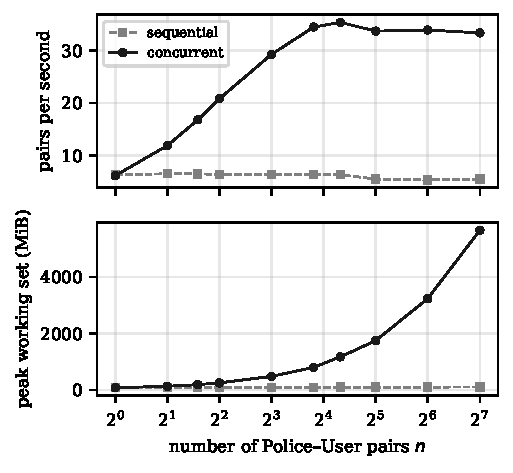
\includegraphics[width=0.92\columnwidth]{generated/fig_e6_scaling.pdf}
\caption{Throughput (top, pairs per second) and peak working set (bottom, MiB) against the number of pairs, median of the repetitions. Concurrent execution scales until the cores are saturated.}
\label{fig:e6}
\end{figure}

\subsection{Payload per Phase (E7)}
Each client uploads 18,776~KiB per assignment (measured after the base64 encoding used by the JSON API), almost all of it key-generation shares and ciphertexts; the garbled circuit and the oblivious transfer together are 8.75~KiB. HTTP headers and JSON framing are not included here.

\subsection{WebAssembly Size and Speed (E9)}\label{sec:e9}
The default build made on the measurement laptop is 11.26~MiB (11,802,642 bytes). Stripping symbols saves little (10.96~MiB), and \code{wasm-opt -Oz} brings the module to 9.86~MiB; it only accepted Go's output with all WebAssembly features enabled. Transfer compression matters far more: brotli reduces the default build to 1.98~MiB and gzip to 2.75~MiB. TinyGo was not installed, so that variant was not attempted.

\textbf{\textit{Why is the module heavy?}} Four ablation builds answer this question. A module with only the Go runtime and \code{syscall/js} is 1.87~MiB; adding only the garbled circuit and the oblivious transfer gives 2.92~MiB; a program that uses single-key BGV is already 11.42~MiB, and adding the multiparty protocols does not increase it (11.40~MiB). Each ablation is a separate small program, so its size depends on which library functions the linker keeps, and it can be slightly larger than the full application. The lattice library, not the multiparty layer or the circuit code, accounts for most of the binary. We know of no other library with a multiparty BGV implementation in WebAssembly, so the comparison is between build configurations of the same library.

\textbf{\textit{Speed.}} The same harness compiled to WebAssembly and run under Node.js v22.21.0 (41 runs) needs 4.1 times the native time for one evaluation. Under Node.js, reading the module takes 4.87~ms [4.71, 5.17] and compiling it 13.4~ms [13.2, 13.9] (median [IQR], 30 runs); V8 compiles functions lazily, so this is mostly validation and understates the real cost. In Chrome, loading and compiling the module until the client is ready takes 48.5~ms [44.4, 51.4] with a cold cache and 31.3~ms [28.9, 35.7] with a warm cache (30 runs each); a Web Worker variant was not measured.

\section{Security Discussion}\label{sec:security}
\subsection{Information Visibility}
The protocol is analyzed under the semi-honest assumption, where each participant follows the protocol specification but tries to obtain information from what it receives. The server sees public key-generation shares, ciphertexts, public E2S shares, garbled data, and the final class, which the Police page stores on the server for the case dashboard; a later version could store only a completion flag. The User sees nothing, whereas the Police see the proximity result.

\subsection{The Server's View on Share Conversion (E11)}
The only plaintext value that the server can compute is the sum of $c_0$ and the public E2S shares, which equals $\Delta$ minus both masks. We found the masks to be effective in hiding $\Delta$.

\subsection{Flooding Margin (E3)}\label{sec:flood}
E2S hides the noise of the ciphertext behind fresh flooding noise. We measured the noise of $\mathrm{Enc}(\Delta)$ after the multiplication and found its standard deviation to be about $2^{36.3}$, while the standard deviation of the flooding noise is $2^{30}$. The flooding noise is therefore smaller than the noise it needs to conceal, by a median of $-6.3$~bits (largest value over all runs: $-6.2$~bits). This does not affect correctness, but it undermines the statistical argument that the public E2S shares reveal nothing about the secret keys or the inputs through the noise. We report it as an open problem: the definition of the margin is ours, and the consequence should be confirmed. Raising the flooding standard deviation to about $2^{76}$, 40~bits above the measured noise, would consume about 46 of the 272.6~bits of noise budget that remain unused, so the fix fits in the deployed parameters.

\subsection{Repeated Queries (E10)}\label{sec:e10}
We simulated an attacker who controls the Police point and the radius and tries to locate a User hidden on a $101 \times 101$ grid (300 random hidden points). With the earlier protocol, which revealed $\Delta$, the median attacker needed 2 queries (maximum 2). Using only the class, a greedy attacker that splits the candidate points in half needs a median of 13 queries (IQR [12, 13], range 4--14; Fig.~\ref{fig:e10}), close to the binary-split estimate of $\log_2 10{,}201 \approx 13.3$. With the quota of three evaluations per hour, this takes a median of 4 hours for one Police account. Since the quota applies per Police--User pair and does not bind queries to a case, collusion lowers this to 2 hours with two Police accounts and to under one hour with five.

\begin{figure}[t]
\centering
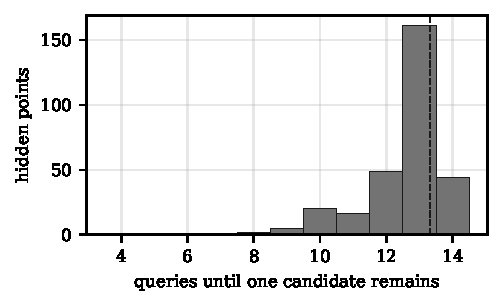
\includegraphics[width=0.92\columnwidth]{generated/fig_e10_queries.pdf}
\caption{Queries an adaptive attacker needs to isolate a hidden grid point when each query returns only the class (simulation, no cryptography). The dashed line is $\log_2 10{,}201$. Most points fall within a few queries of the estimate because a circle splits the candidate set almost evenly.}
\label{fig:e10}
\end{figure}

\subsection{Cheating Garbler (E12)}
The evaluator cannot verify that a garbled AND table implements AND. In a unit test that is not part of the application, a garbler rewrites the 16 AND gates of the ``$\Delta = 0$'' chain so that the second output bit equals one chosen bit of $\Delta \bmod t$; 17 such garblings recovered $\Delta \bmod t$ exactly in 300 of 300 trials, and the evaluator reported no error. A second test forces the output to outside for every input by changing the decode bits. With the roles of the prototype (the User garbles), this is an integrity attack in which a dishonest User decides which class the Police see. The first test shows that the function evaluated is whatever the garbler decides, which is why the semi-honest assumption cannot be dropped.

\subsection{Out-of-Range Inputs (E2)}
The server cannot know whether an encrypted coordinate lies in $[0, 100]$. According to Section~\ref{sec:e2}, any input that pushes $\Delta$ beyond $\pm 32{,}768$ flips the class, so a modified client can force a wrong answer without being detected; the result is therefore not evidence, since the User's input cannot be verified.

\subsection{Human in the Loop}
A query is created by an authorized Police account, and the computation only begins after the User clicks the button that encrypts their location. The User's interface states that the answer will be delivered to the Police only. Hence, the User must actively approve each computation. However, the User cannot see the Police point or the motive of the inquiry, and the User is not told the outcome. Who may open a case and how this is audited is outside the prototype.

\subsection{Security Limitations}
The design does not protect against a party that deviates from the protocol, against a server that distributes modified client code, or against repeated queries. To mitigate the last point, the server allows one evaluation per assignment and three evaluations per Police--User pair per hour.

\section{Conclusions}\label{sec:concl}
In this paper we presented UMBRA, a web application that determines whether a user is inside a certain radius using cryptographic techniques, without revealing the user's location, only one class per query.

The user's location is encrypted on the user's own device, and the computation is carried out on the server on the encrypted locations without obtaining any information about the original data, including whether the user is inside the radius or not.

The method was tested and showed good performance and accuracy: in 10,011 tests, the result always coincided with the result computed beforehand in plaintext. The cryptographic operations take less than a second on the tested laptop, and the full query in the browser takes about seven seconds, most of it spent waiting for messages.

Our answer to the research question is therefore yes: a service can deliver a useful result from data it never sees.

The relevance of this project comes from the constant collection of location data that is valuable for many services, while not everybody is willing to share it and disclose their private information, as the Gravy Analytics case showed~\cite{ftc,tc}. Our design allows a service to keep its business logic, whether a certain person visited a particular place during an investigation, a delivery reached a certain area, or a user is within the service area, while every person keeps their precise location on a personal device. The approach can also be extended to other sensitive numbers, such as health or financial data, whenever a service only needs a yes or no answer.

The system has limitations. It guarantees privacy when both participants use the application correctly, but a participant who manipulates the application can change the outcome. Every query also gives a clue: a participant who asks repeatedly, thirteen times in our simulation, can find out the location of the user. Limiting the number of queries helps, but it is not enough.

The next steps are to protect the system against participants who cheat and to make it faster in the browser, for example by replacing the one-second polling with messages pushed by the server.

\begin{thebibliography}{99}
\bibitem{bgv} Z.~Brakerski, C.~Gentry, and V.~Vaikuntanathan, ``Fully homomorphic encryption without bootstrapping,'' Cryptology ePrint Archive, Paper 2011/277, 2011. [Online]. Available: \url{https://eprint.iacr.org/2011/277}
\bibitem{mouchet} C.~Mouchet, J.~Troncoso-Pastoriza, J.-P. Bossuat, and J.-P. Hubaux, ``Multiparty homomorphic encryption from ring-learning-with-errors,'' \emph{Proc. Privacy Enhancing Technologies}, vol.~2021, no.~4, pp.~291--311, 2021, doi: 10.2478/popets-2021-0071.
\bibitem{yao86} A.~C.-C. Yao, ``How to generate and exchange secrets,'' in \emph{Proc. 27th Annu. Symp. Foundations of Computer Science (FOCS)}, 1986, pp.~162--167, doi: 10.1109/SFCS.1986.25.
\bibitem{bhr12} M.~Bellare, V.~T. Hoang, and P.~Rogaway, ``Foundations of garbled circuits,'' Cryptology ePrint Archive, Paper 2012/265 (proceedings version in ACM CCS 2012). [Online]. Available: \url{https://eprint.iacr.org/2012/265}
\bibitem{bmr90} D.~Beaver, S.~Micali, and P.~Rogaway, ``The round complexity of secure protocols,'' in \emph{Proc. 22nd ACM Symp. Theory of Computing (STOC)}, 1990, pp.~503--513, doi: 10.1145/100216.100287.
\bibitem{freexor} V.~Kolesnikov and T.~Schneider, ``Improved garbled circuit: Free XOR gates and applications,'' in \emph{Proc. ICALP 2008}, LNCS vol.~5126, Springer, pp.~486--498, doi: 10.1007/978-3-540-70583-3\_40.
\bibitem{chouorlandi} T.~Chou and C.~Orlandi, ``The simplest protocol for oblivious transfer,'' Cryptology ePrint Archive, Paper 2015/267 (LATINCRYPT 2015). [Online]. Available: \url{https://eprint.iacr.org/2015/267}
\bibitem{lattigo} Tune Insight SA, ``Lattigo v6.2.0.'' [Online]. Available: \url{https://github.com/tuneinsight/lattigo}
\bibitem{hestd} HomomorphicEncryption.org, ``Homomorphic Encryption Standard,'' Nov. 2018. [Online]. Available: \url{https://homomorphicencryption.github.io/assets/HomomorphicEncryptionStandard2018.pdf}
\bibitem{ftc} Federal Trade Commission, ``FTC takes action against Gravy Analytics, Venntel for unlawfully selling location data tracking consumers to sensitive sites,'' press release, Dec.~3, 2024. [Online]. Available: \url{https://www.ftc.gov/news-events/news/press-releases/2024/12/ftc-takes-action-against-gravy-analytics-venntel-unlawfully-selling-location-data-tracking-consumers}
\bibitem{tc} Z.~Whittaker, ``A breach of Gravy Analytics' huge trove of location data threatens the privacy of millions,'' \emph{TechCrunch}, Jan.~13, 2025. [Online]. Available: \url{https://techcrunch.com/2025/01/13/gravy-analytics-data-broker-breach-trove-of-location-data-threatens-privacy-millions/}
\bibitem{zhong07} G.~Zhong, I.~Goldberg, and U.~Hengartner, ``Louis, Lester and Pierre: Three protocols for location privacy,'' in \emph{Privacy Enhancing Technologies (PET 2007)}, LNCS vol.~4776, Springer, 2007, pp.~62--76, doi: 10.1007/978-3-540-75551-7\_5.
\bibitem{narayanan11} A.~Narayanan, N.~Thiagarajan, M.~Lakhani, M.~Hamburg, and D.~Boneh, ``Location privacy via private proximity testing,'' in \emph{Proc. Network and Distributed System Security Symp. (NDSS)}, San Diego, CA, USA, 2011.
\bibitem{sedenka14} J.~\v{S}ed\v{e}nka and P.~Gasti, ``Privacy-preserving distance computation and proximity testing on Earth, done right,'' in \emph{Proc. 9th ACM Symp. Information, Computer and Communications Security (ASIA CCS)}, 2014, pp.~99--110, doi: 10.1145/2590296.2590307.
\bibitem{hallgren15} P.~Hallgren, M.~Ochoa, and A.~Sabelfeld, ``InnerCircle: A parallelizable decentralized privacy-preserving location proximity protocol,'' in \emph{Proc. 13th Annu. Conf. Privacy, Security and Trust (PST)}, 2015, doi: 10.1109/PST.2015.7232947.
\bibitem{dp3t} C.~Troncoso \emph{et al.}, ``Decentralized privacy-preserving proximity tracing,'' \emph{IEEE Data Eng. Bull.}, vol.~43, no.~2, pp.~36--66, 2020. [Online]. Available: \url{https://arxiv.org/abs/2005.12273}
\end{thebibliography}

\appendices
\section{Functional Evidence}\raggedright\label{app:evidence}
Fig.~\ref{fig:appendix} shows the pages captured by an automated script (Appendix~\ref{app:repro}), which runs a throw-away copy of the application and drives two tabs of headless Chrome. The interface of the prototype is in Spanish: DENTRO DEL RADIO is inside, EXACTAMENTE EN EL LIMITE is boundary and FUERA DEL RADIO is outside. The observed texts are recorded with the other results.

\begin{figure*}[t]
\centering
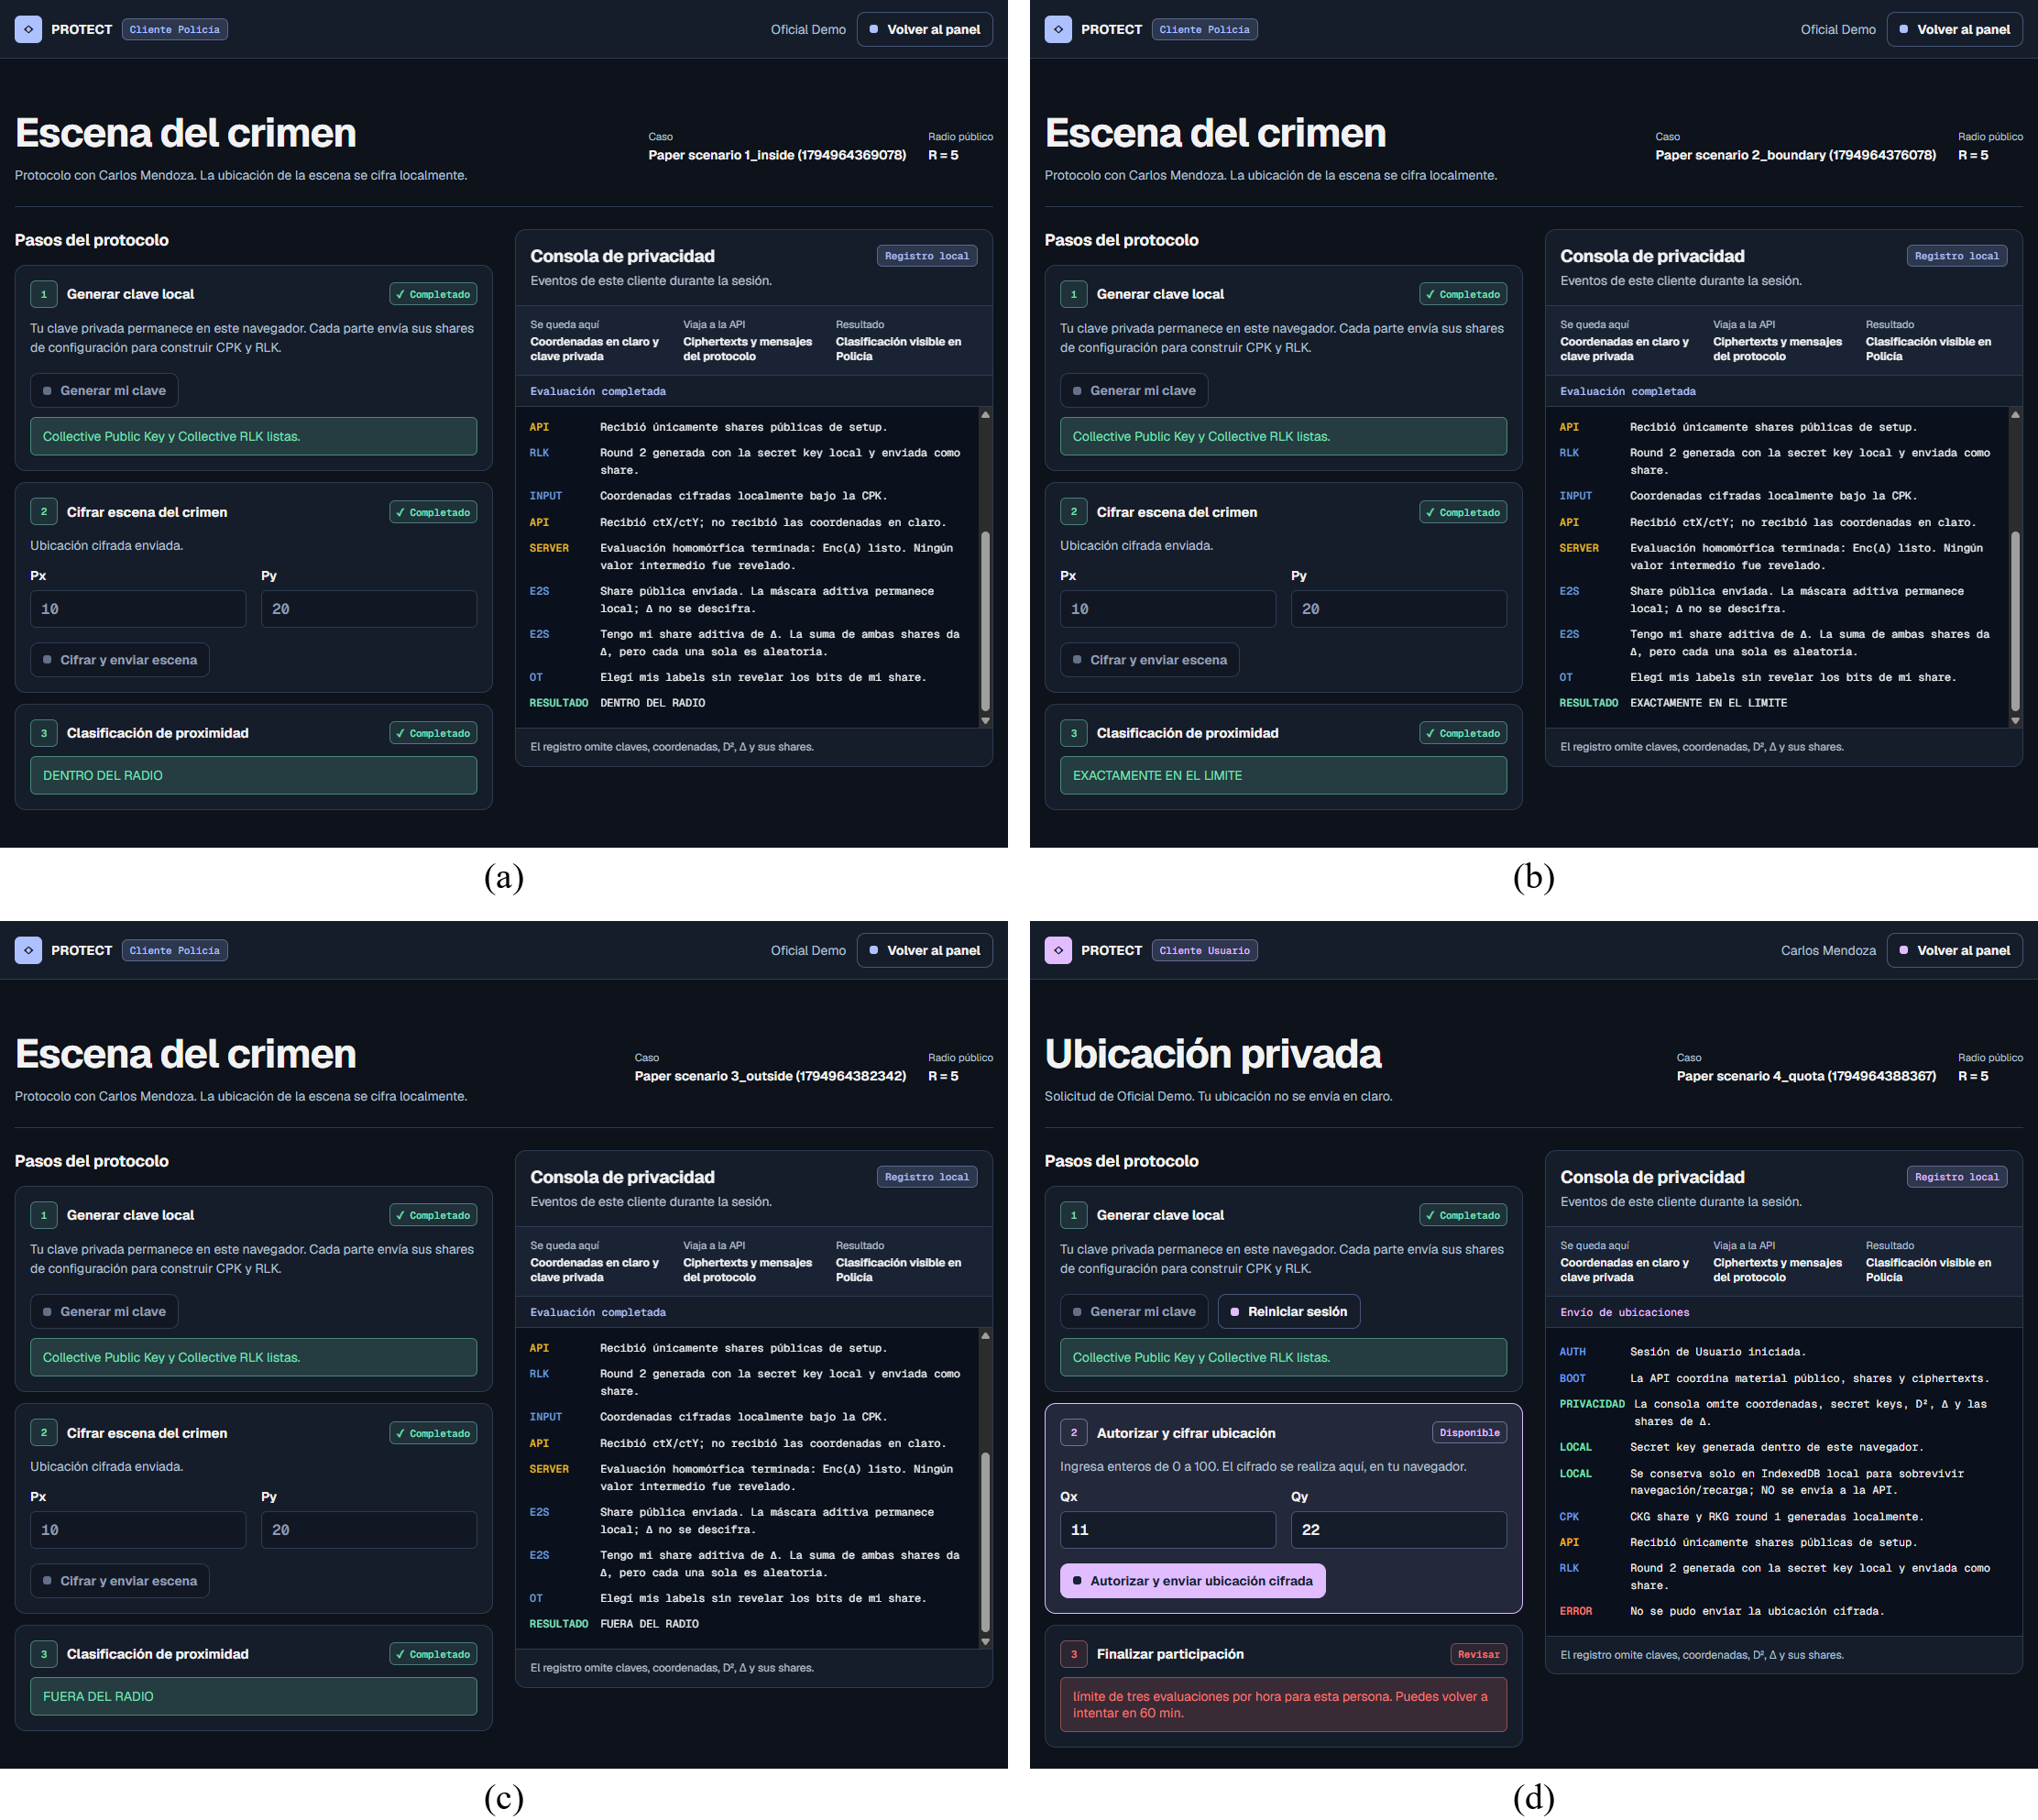
\includegraphics[width=0.92\textwidth]{figures/fig4_appendix_new.png}
\caption{Browser evidence for the four scenarios, all with $P = (10, 20)$ and $R = 5$. (a)~Police page, $U = (11, 22)$, $\Delta = -20$: expected inside. (b)~Police page, $U = (13, 24)$, $\Delta = 0$: expected boundary. (c)~Police page, $U = (14, 24)$, $\Delta = 7$: expected outside. (d)~User page, fourth evaluation of the same pair within one hour: quota error.}
\label{fig:appendix}
\end{figure*}

\section{Reproducibility}\label{app:repro}
\raggedright
Repository: \url{https://github.com/albertolopezb/fhe-garbled-circuits}, commit \code{e15231d} on branch \code{paper/rerun-20261117}, where \code{bash bench/rerun\_all.sh} runs every step below in order. Hardware and software are recorded in \code{results/hardware.json}. From the repository root in Git Bash:
{\footnotesize
\begin{verbatim}
GOTOOLCHAIN=go1.26.0 go build -o bin/bench.exe \
    ./cmd/bench
./bin/bench.exe hardware
./bin/bench.exe e1 -seed 1 -n 10000
./bin/bench.exe e2
./bin/bench.exe e3 -seed 1 -n 1000
./bin/bench.exe e4 -n 1000 -reps 30 -workers 8
./bin/bench.exe e5a ; ./bin/bench.exe e5b
./bin/bench.exe e6 ; ./bin/bench.exe e7
./bin/bench.exe e11 -n 1000
GOTOOLCHAIN=go1.26.0 go test ./bench   # E12
bash bench/e9_wasm.sh
python bench/e10_leakage.py --seed 1 --points 300
bash bench/e9_node.sh
bash bench/browser_scenarios.sh
node bench/browser_bench.mjs heat 5
node bench/browser_bench.mjs profile 10
node bench/browser_bench.mjs load 30
node bench/browser_bench.mjs robust
python paper/make_assets.py
\end{verbatim}
}
\noindent Raw logs and replaced result files are kept in \code{results/raw/}. The security-table check is recorded in \code{results/SECURITY\_CHECK.md}.

\end{document}
